% Бүлэг 3
\chapter{Улаанбаатар хотын дугуйн замын crowd-sourcing веб системийн зохиомж ба хөгжүүлэлт} % Зарим нэг зөвлөмж
\label{Chapter3} % Энэ бүлэг рүү ишлэл хийх бол \ref{Chapter3} командыг ашигла

\section{Системийн архитектур}
\paragraph{}
Улаанбаатар хотын дугуйн замын crowd-sourcing веб систем нь Back-end болон Front-end гэсэн үндсэн хоёр хэсгээс бүрдэнэ. Зураг \ref{fig:sys-arch} -д үзүүлсний дагуу Front-end хэсэг нь хэрэглэгчид харагдаж, хэрэглэгчтэй харилцах хэсэг бөгөөд хэрэглэгчийн оролтын мэдээллийг (сегмент тэмдэглэгээ, POI байршил, маршрутын эхлэл/төгсгөл цэг) авч Back-end хэсгээс гаргасан REST API сервисийг ашиглан Back-end хэсэг рүү хүсэлт явуулж, хариуг аван хэрэглэгчийг гаралтын мэдээллээр (өнгөтэй сегмент, POI marker, аюулгүй маршрут) хангана. Back-end хэсгийн хувьд системийн логик үйл ажиллагааг хангаж ажилладаг бөгөөд Django фреймворк дээр хөгжүүлэгдсэн. Хэрэглэгчийн нэвтрэлт (JWT), бүртгэл, замын сегмент тэмдэглэх, POI байрлуулах, crowd aggregation -ыг тооцоолох, ухаалаг маршрут гаргахтай холбоотой сервисүүдийг гаргаж, OpenStreetMap газрын зургийг үзүүлэгч Leaflet, маршрут тооцооллын 3-дагч талын сервис болох OSRM, хэрэглэгчдийн мэдээлэл болон тэдгээрт хамааралтай сегмент, POI, нэгтгэлийн өгөгдлийг хадгалах MySQL өгөгдлийн сантай ажиллана.
\begin{figure}[H]
    \centering
    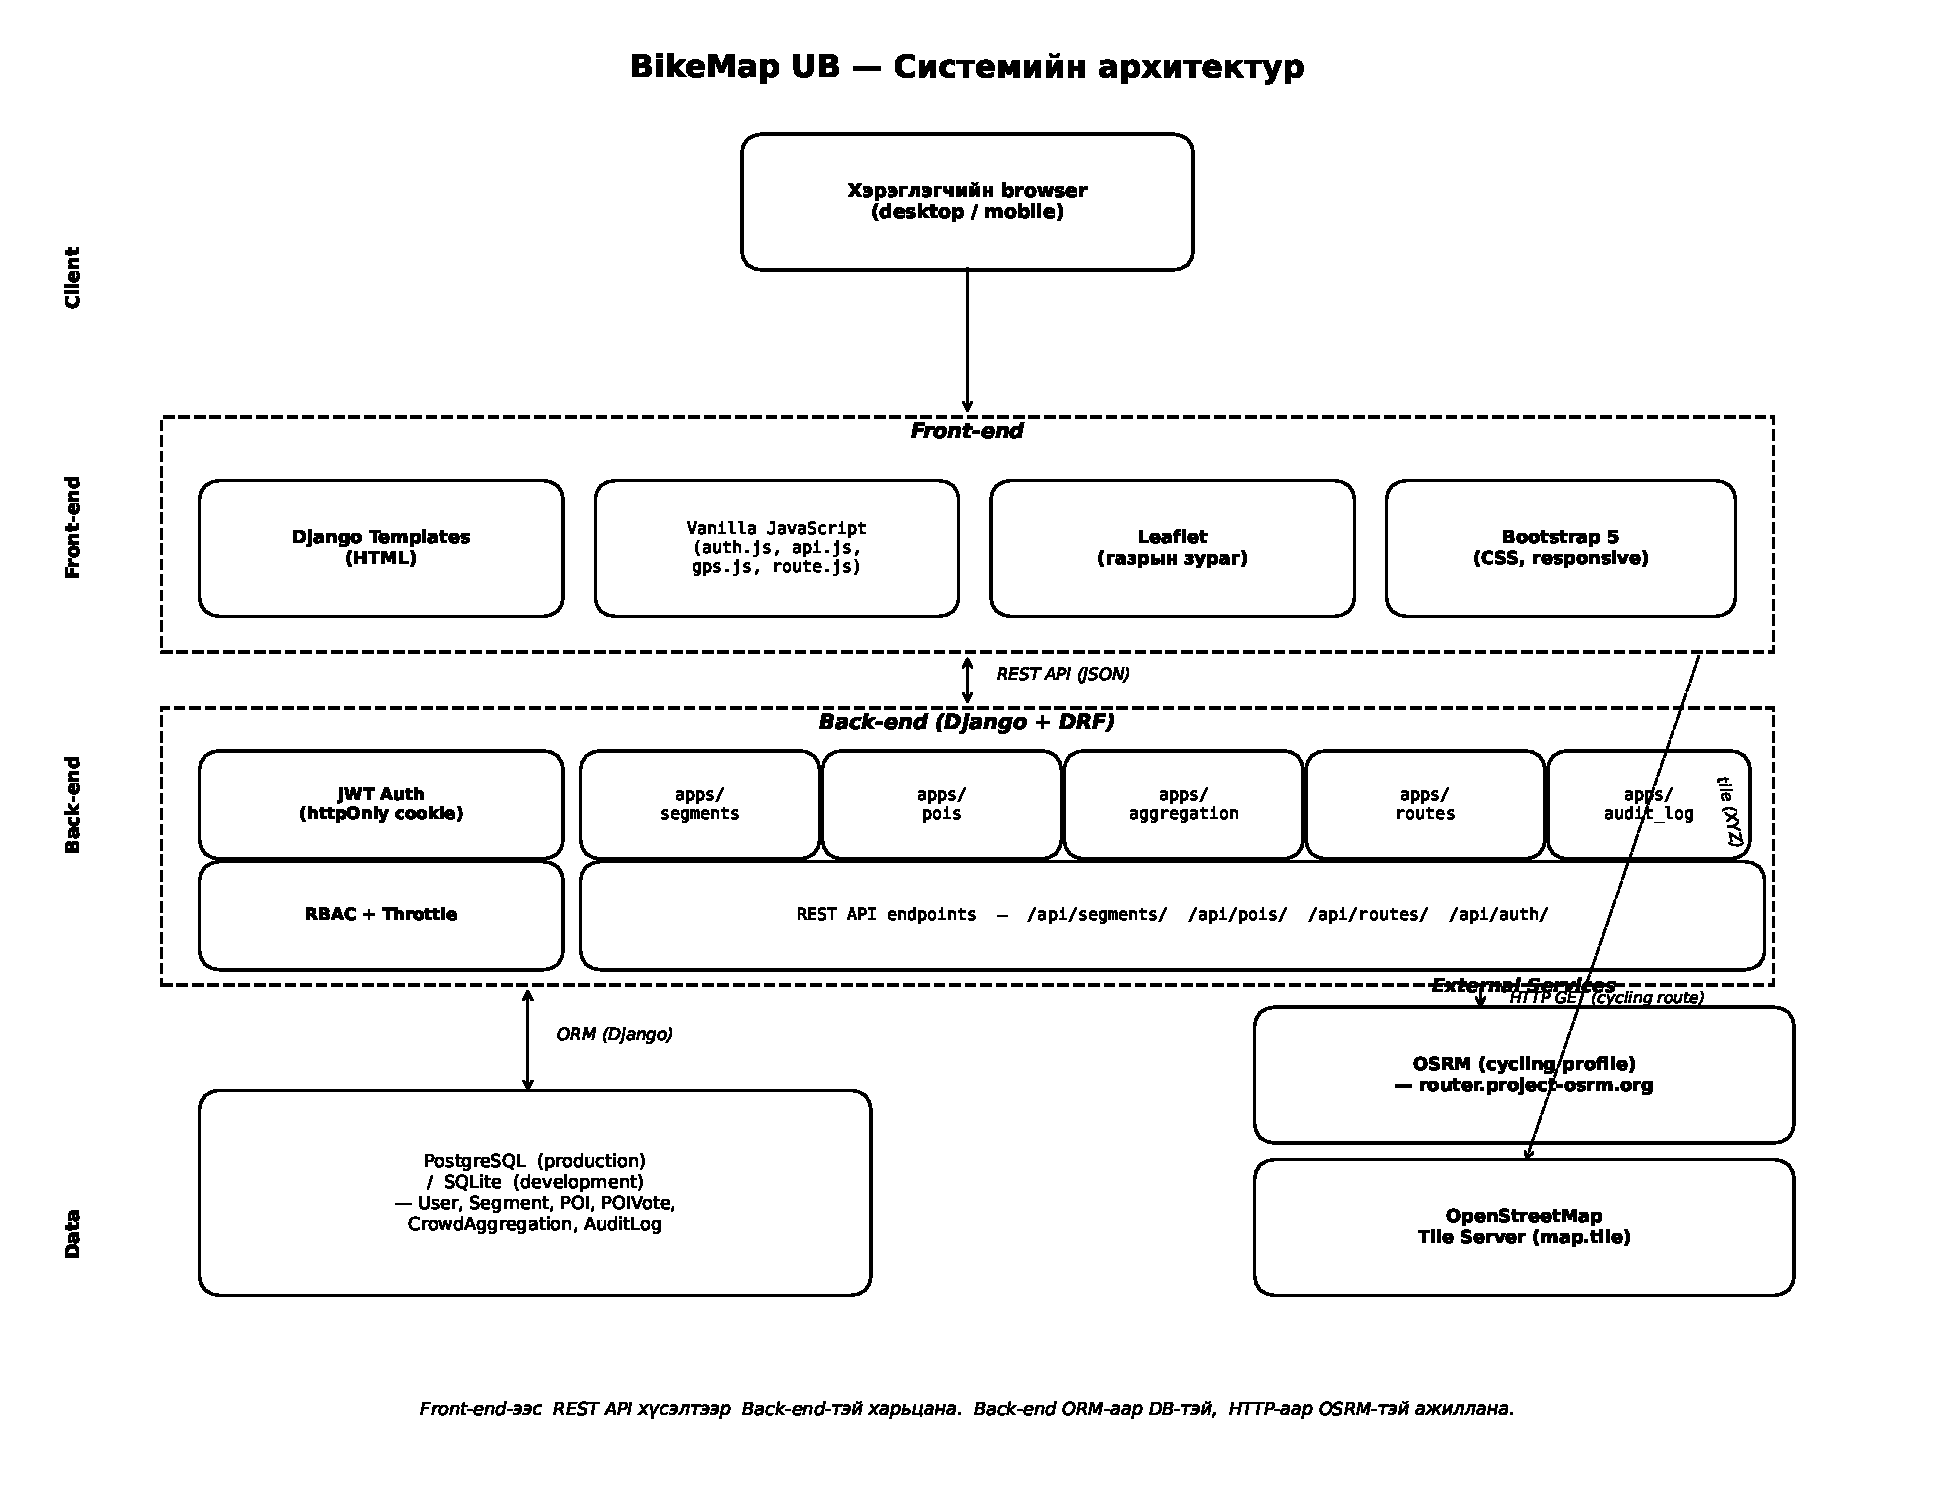
\includegraphics[scale=0.9]{Figures/chapter3/arch-diagram.pdf}
    \caption{Системийн архитектур}
    \label{fig:sys-arch}
\end{figure}

\section{Зохиомжийн шатны класс диаграмм}
\paragraph{} Дугуйн замын crowd-sourcing веб системийн зохиомжийн шатны класс диаграммд \say{control} төрлийн \say{Хэрэглэгч}, \say{Сегмент}, \say{POI}, \say{Crowd Aggregation}, \say{Smart Route}, \say{Бүртгэл} гэсэн 6 класс, \say{entity} төрлийн \say{Хэрэглэгчийн мэдээлэл}, \say{Сегментийн мэдээлэл}, \say{POI мэдээлэл}, \say{Aggregation мэдээлэл} гэсэн 4 класс, \say{boundary} төрлийн \say{Газрын зургийн дэлгэц}, \say{Бүртгэлийн дэлгэц}, \say{Нэвтрэх дэлгэц}, \say{POI дэлгэрэнгүй дэлгэц}, \say{Маршрутын дэлгэц}, \say{Профайлын дэлгэц}, \say{Админы dashboard дэлгэц} гэсэн 7 класс буюу нийт 17 классын аттрибут болон операторуудыг тодорхойлсон. Зураг \ref{fig:z-class} -д тэдгээр классуудын стерео төрлийг тодорхойлж, класс хоорондын холбоо хамаарлыг ассосиэйшн болон бүрдмэл холбоо хамаарлаар дүрсэлж, зарим класс хоорондын холбоо хамааралд ашиглалтын хараат байдлыг дүрсэлсэн.
\begin{figure}[!h]
    \centering
    % 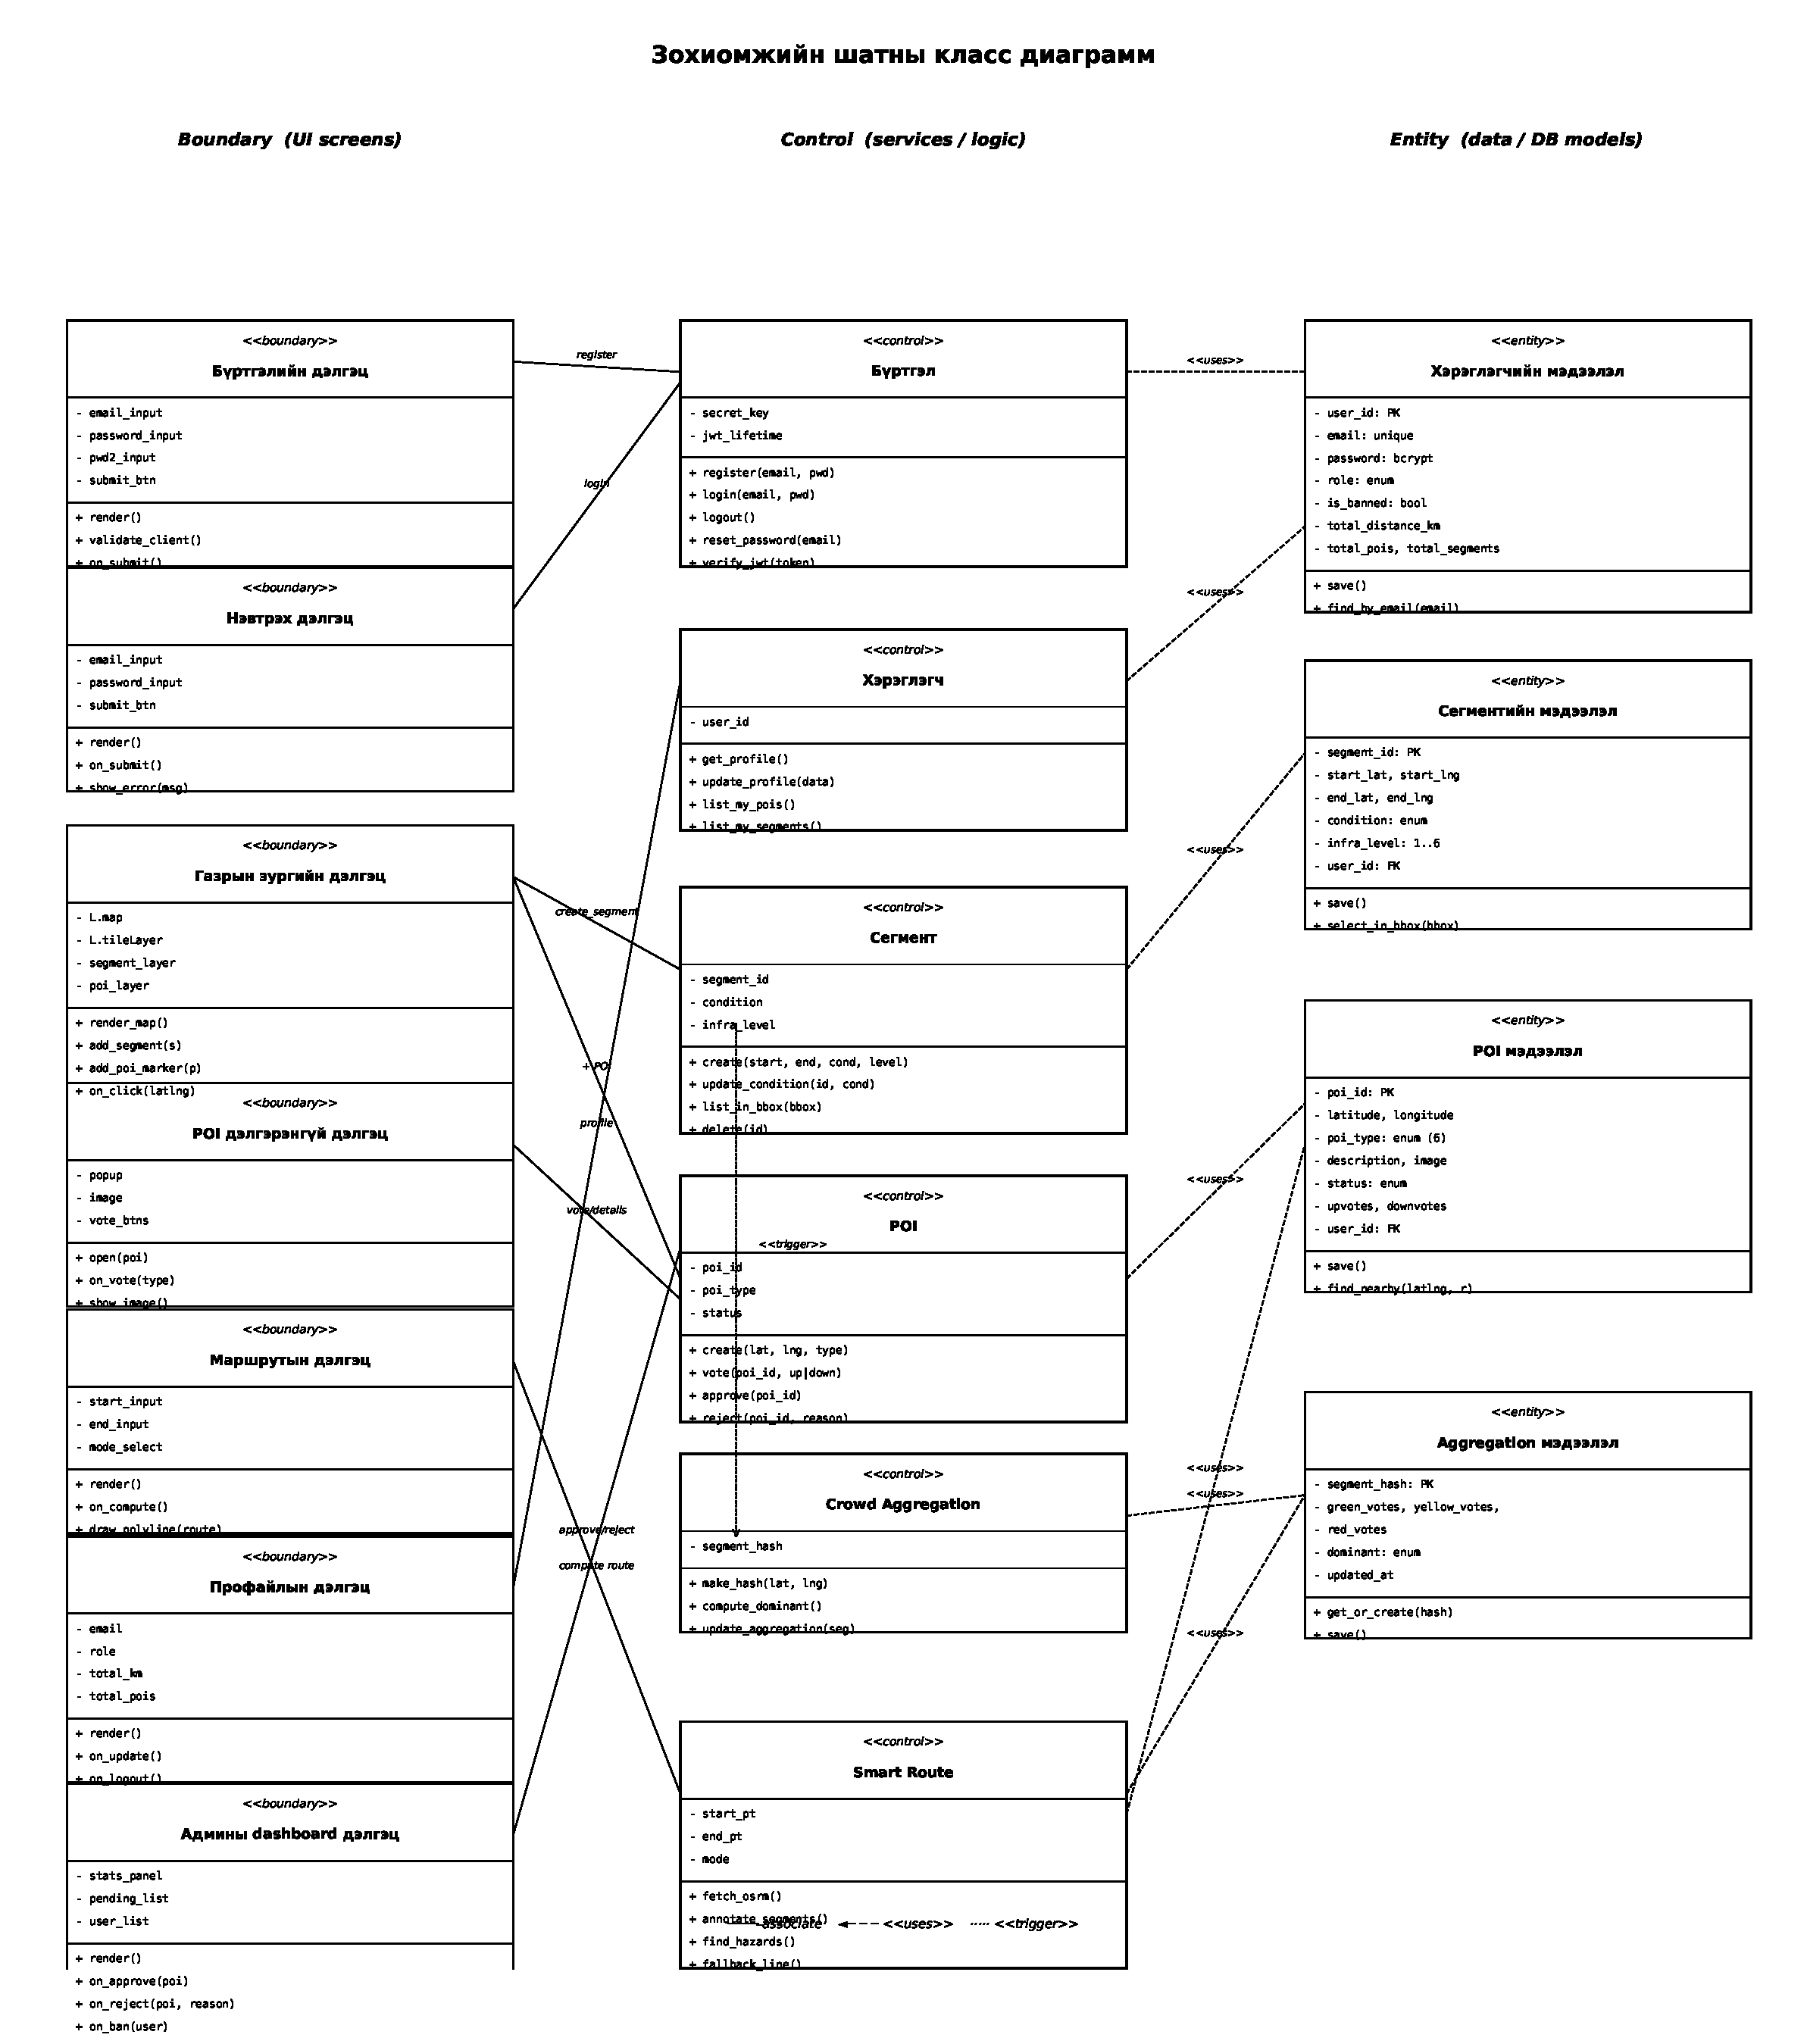
\includegraphics[scale=0.4, angle = 90]{Figures/chapter3/s_class_diagram.jpg} % auto-commented: missing file
    \caption{Класс диаграмм}
    \label{fig:z-class}
\end{figure}

\section{Өгөгдлийн ерөнхий схем }
\paragraph{} Дугуйн замын crowd-sourcing веб системийн өгөгдлийн сан нь Хэрэглэгч (User), Сегмент (Segment), POI болон Crowd Aggregation гэсэн дөрвөн үндсэн хүснэгтийг агуулна. Хэрэглэгч хүснэгт нь системд бүртгүүлсэн хэрэглэгчдийн имейл, нууц үгийн bcrypt hash, ролийн төрөл (зочин/хэрэглэгч/админ), бүртгэлийн огноо болон хэрэглэгчийн ID-г анхдагч түлхүүрээр хадгална. Сегмент хүснэгт нь сегментийн ID-г анхдагч түлхүүрээр, эхлэх ба дуусах өргөрөг/уртраг (DECIMAL(9,6)), нөхцлийн ангилал (green/yellow/red), дэд бүтцийн зэрэглэл (1-6), Create Segment-ээр үүсгэсэн эсэх (is\_created), оруулсан хэрэглэгчийн ID-г гадаад түлхүүрээр хадгална. POI хүснэгт нь POI-ийн ID-г анхдагч түлхүүрээр, өргөрөг, уртраг, төрөл (Danger / No Bike Lane / Road Damage / Parking Problem / Bike Repair / Bike Parking), тайлбар, зургийн URL, статус (pending/approved/rejected), upvote, downvote тоо, оруулсан огноо болон хэрэглэгчийн ID-г гадаад түлхүүрээр хадгална. Crowd Aggregation хүснэгт нь сегментийн hash утгыг түлхүүрээр, ногоон/шар/улаан саналуудын тоо, давамгай нөхцөл болон сүүлд шинэчилсэн огноог хадгална. Зураг \ref{fig:erd} -д системийн хөгжүүлэлтийн хүрээнд үүсгэсэн өгөгдлийн сангийн "Хэрэглэгч", "Сегмент", "POI", "Crowd Aggregation" гэсэн хүснэгтүүд, тэдгээрийн аттрибутууд болон тэдгээр хүснэгтүүдийн хооронд "1 : олон" харьцаагаар дүрслэгдсэнийг харуулж байна.
\begin{figure}[H]
    \centering
    % 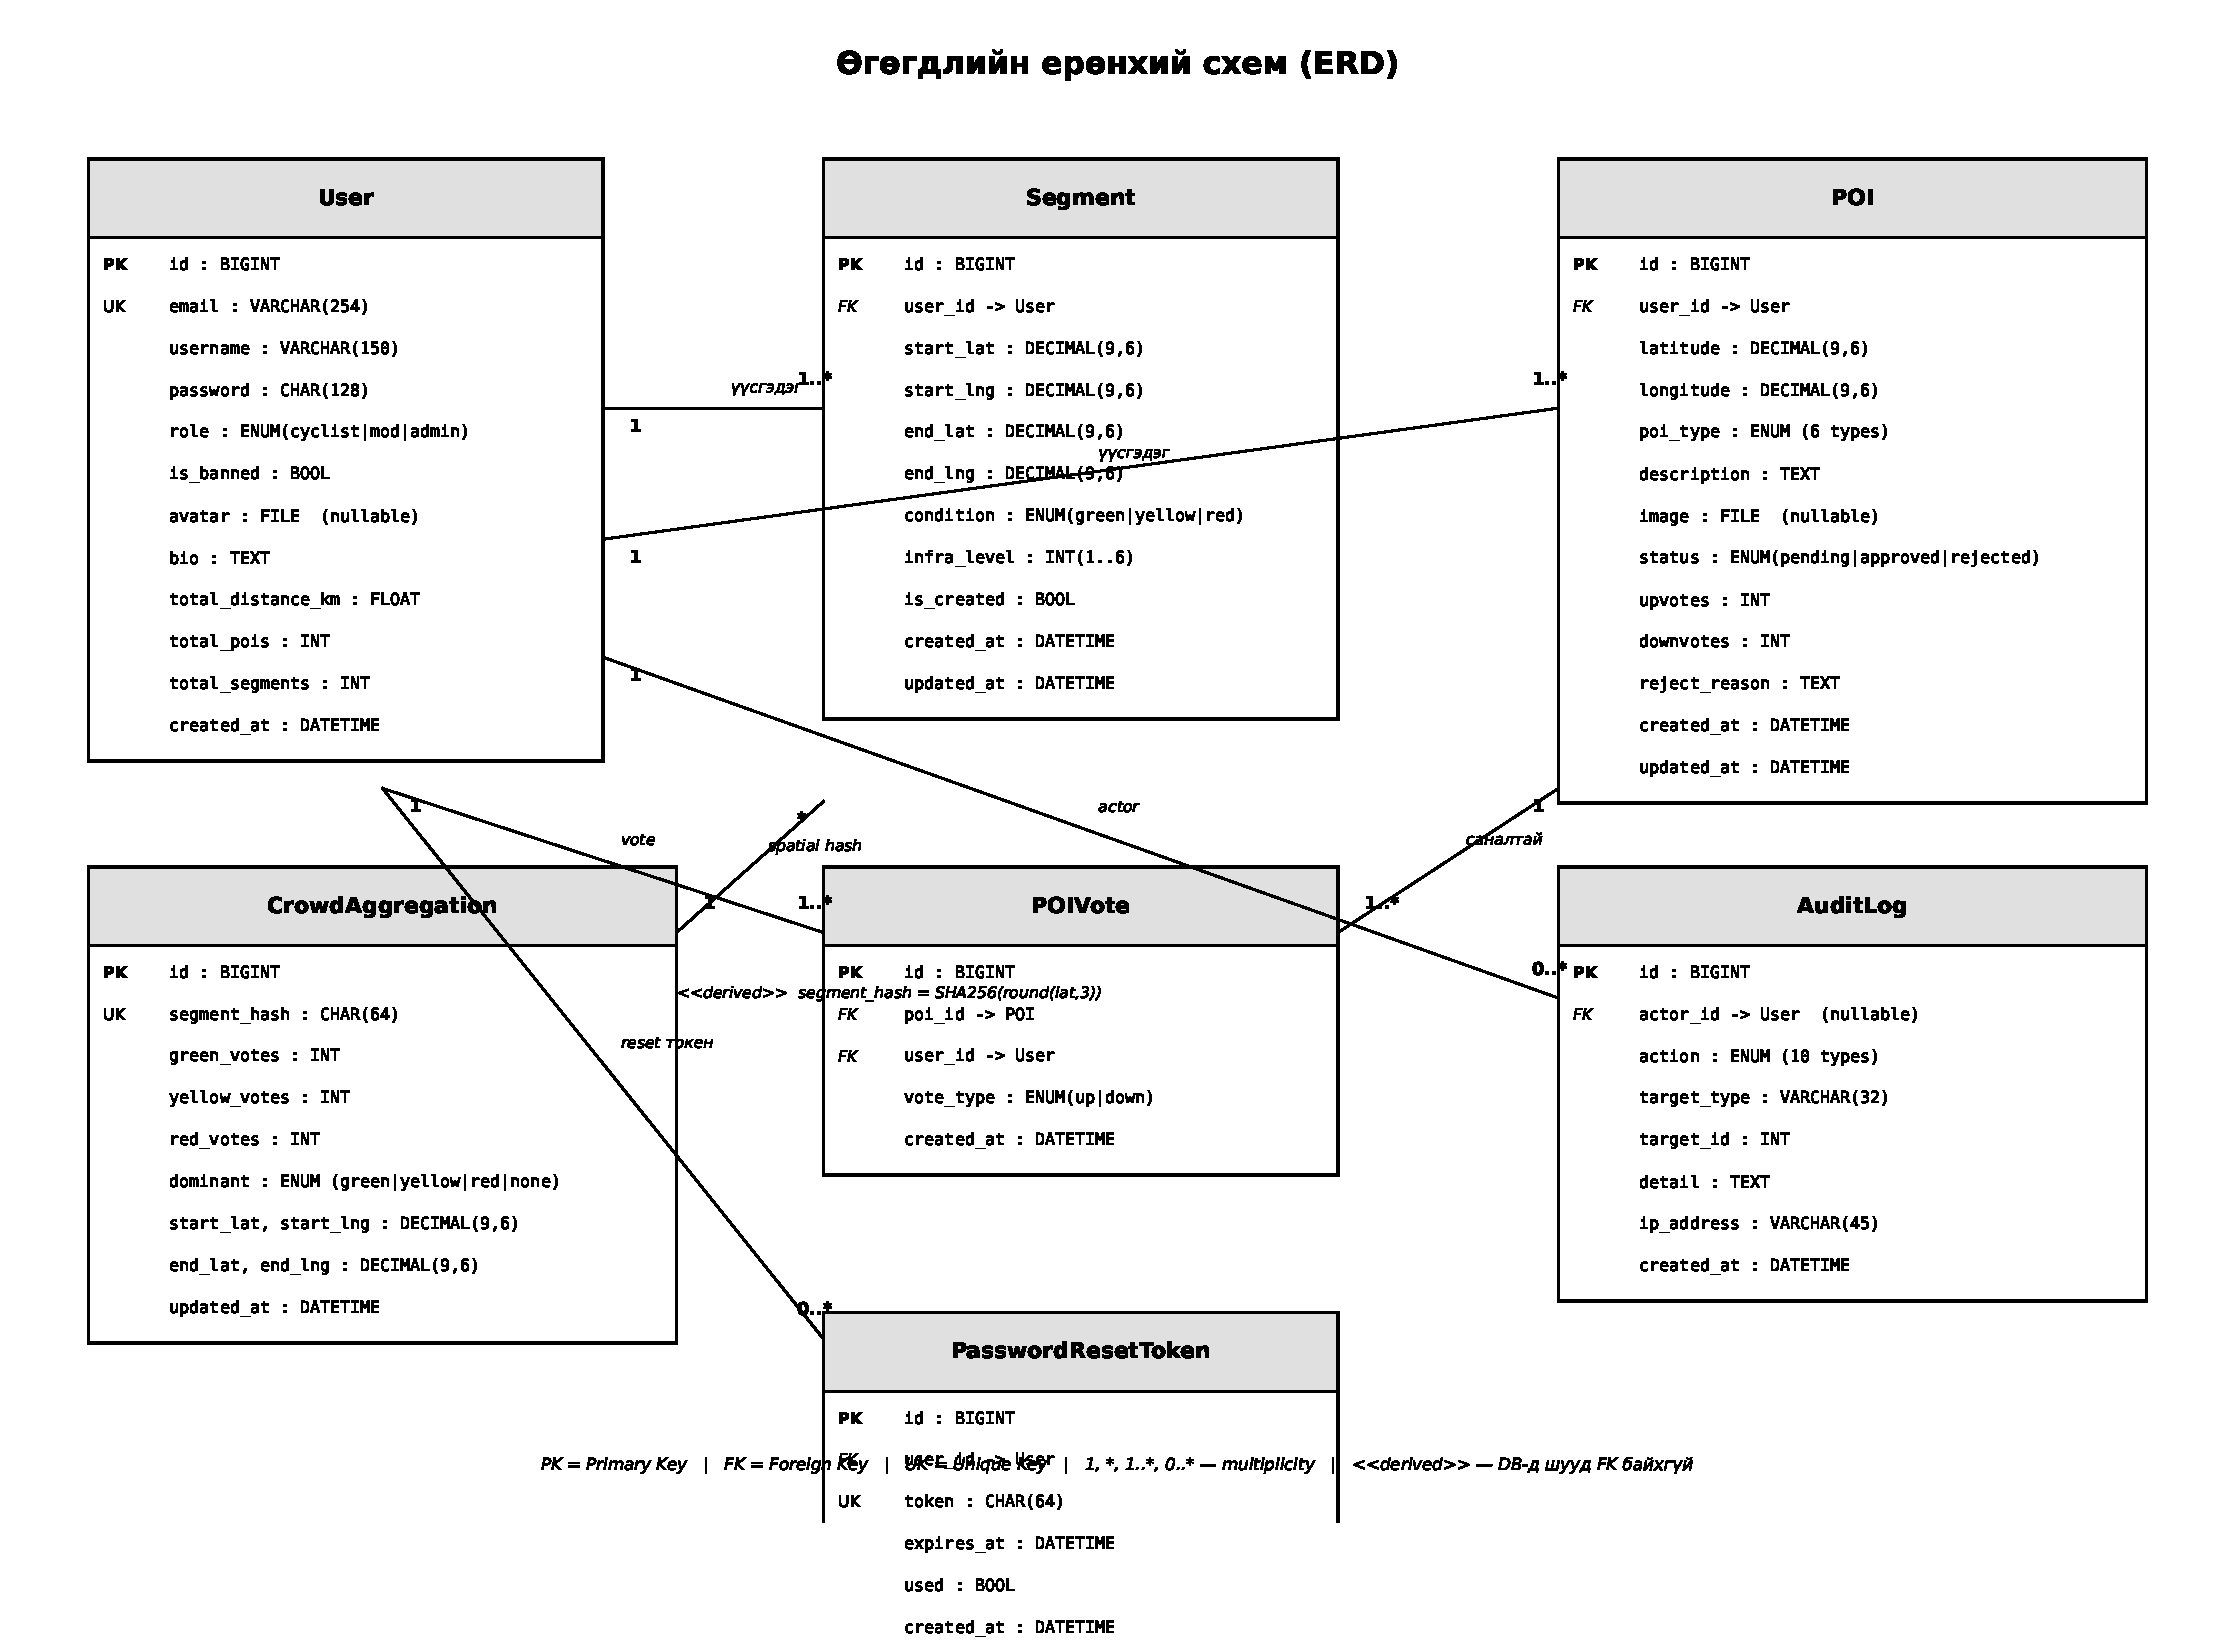
\includegraphics[scale=0.8]{Figures/chapter3/erd.PNG} % auto-commented: missing file
    \caption{Өгөгдлийн ерөнхий схем}
    \label{fig:erd}
\end{figure}

\section{Системийн прототип}
\paragraph{} Системийн үндсэн хуудас, бүртгүүлэх болон нэвтрэх хуудас, газрын зураг дээр сегмент тэмдэглэх ба POI байрлуулах, маршрут гаргах, хэрэглэгчийн мэдээллээ шинэчлэх болон оруулсан POI/route-уудаа удирдах хуудаснуудын прототип загварыг дүрслэн харуулна.
\par \noindent Зураг \ref{fig:proto_map} -д crowd-sourcing вебийн хэрэглэгчийн бүртгэлээр ороогүй байх үеийн газрын зургийн нүүр хуудас харагдаж байна. Тус хуудсанд crowd aggregation -аар тооцоологдсон сегментүүд өнгөөр (ногоон/шар/улаан) дүрслэгдсэн, POI-ууд нь марker -аар харагдаж байна.
\begin{figure}[!h]
    \centering
    % \includegraphics[scale=0.305]{Figures/chapter3/Frame 1.pdf} % auto-commented: missing file
    \caption{Газрын зургийн нүүр хуудасны прототип}
    \label{fig:proto_map}
\end{figure}
\newline
\par \noindent Зураг \ref{fig:proto_map} -д үзүүлсэн хэрэглэгчийн бүртгэлээр нэвтрээгүй байх үеийн нүүр хуудасны толгой хэсэгт байрлах "Бүртгүүлэх" лабелийг дарснаар тус хуудас гарч ирнэ. Зураг \ref{fig:proto_signup} -д хэрэглэгчийн бүртгэлийн мэдээллийг (имейл, нууц үг) авч бүртгэл үүсгэх хуудсыг харуулж байна.
\begin{figure}[H]
    \centering
    % \includegraphics[scale=0.23]{Figures/chapter3/Frame 2.pdf} % auto-commented: missing file
    \caption{Бүртгэл үүсгэх хуудасны прототип}
    \label{fig:proto_signup}
\end{figure}
\par \noindent Зураг \ref{fig:proto_route} -д хэрэглэгч эхлэл болон төгсгөлийн цэгийг сонгож аюулгүй маршрут гаргах хуудасны прототип харагдаж байна. Хэрэглэгч "Аюулгүй" эсвэл "Хурдан" гэсэн маршрутын төрлийг сонгож болно.
\begin{figure}[H]
    \centering
    % \includegraphics[scale=0.23]{Figures/chapter3/Frame 3.pdf} % auto-commented: missing file
    \caption{Маршрут гаргах хуудасны прототип}
    \label{fig:proto_route}
\end{figure}
% \clearpage

\section{Хөгжүүлсэн системийн интерфейс}
\paragraph{} Хөгжүүлэгдсэн системийн газрын зургийн нүүр хуудас, нэвтрэх, бүртгүүлэх, сегмент тэмдэглэх, POI байрлуулах, маршрут гаргах хуудаснууд болон хэрэглэгчийн профайл, админы dashboard хуудсыг энэ хэсэгт тайлбарлана.
\par \noindent Зураг \ref{fig:home} -д харуулсан интерфейстэй хуудас нь хэрэглэгчийг веб хуудас руу хэрэглэгчийн бүртгэлгүйгээр хандах үед харагдана. Газрын зургийн дээр crowd aggregation -аас гаргасан давамгай нөхцлийн дагуу сегментүүд ногоон/шар/улаан өнгөтэй харагдана. POI-ууд нь марker -аар харагдаж, дарснаар дэлгэрэнгүй мэдээлэл popup хэлбэрээр гарч ирнэ.
\begin{figure}[H]
    \centering
    % \includegraphics[scale=0.4]{Figures/chapter3/home.pdf} % auto-commented: missing file
    \caption{Газрын зургийн нүүр хуудасны интерфейс}
    \label{fig:home}
\end{figure}
\par \noindent Зураг \ref{fig:login} -д системийн нэвтрэх хуудасны интерфейсийг харуулсан. Бүртгэлтэй хэрэглэгч имейл хаяг болон нууц үгээ оруулаад "Нэвтрэх" товчийг дарж системд нэвтэрнэ. Систем JWT токен үүсгэн front-end рүү буцаана. Хэрэглэгчийн оруулсан имейл хаяг бүртгэлгүй эсвэл нууц үг буруу тохиолдолд алдааны мессежийг хэрэглэгчид харуулна. Хэрэв бүртгэлгүй бол "Одоо бүртгүүлэх" гэсэн лабелийг дарж бүртгүүлэх хуудас руу очиж болно.
\begin{figure}[H]
    \centering
    % \includegraphics[scale=0.4]{Figures/chapter3/login.pdf} % auto-commented: missing file
    \caption{Нэвтрэх хуудасны интерфейс}
    \label{fig:login}
\end{figure}
\par \noindent Зураг \ref{fig:segment} -д сегментийн нөхцөл тэмдэглэх хуудасны интерфейс харагдаж байна. Бүртгэлтэй хэрэглэгч "Сегмент тэмдэглэх" товчийг дарсны дараа газрын зураг дээр эхлэл болон төгсгөл цэг сонгоно. Дараа нь өнгөний сонголт UI гарч ирнэ — ногоон, шар, улаан гэсэн гурван сонголтын аль нэгийг сонгож хадгална.
\begin{figure}[H]
    \centering
    % \includegraphics[scale=0.4]{Figures/chapter3/segment.pdf} % auto-commented: missing file
    \caption{Сегментийн нөхцөл тэмдэглэх хуудасны интерфейс}
    \label{fig:segment}
\end{figure}
\par \noindent Зураг \ref{fig:poi} -д POI байрлуулах хуудасны интерфейсийг харуулсан. Хэрэглэгч газрын зураг дээр цэг сонгоход POI төрөл сонгох UI гарна (Danger / No Bike Lane / Road Damage / Parking Problem / Bike Repair / Bike Parking). Хэрэглэгч төрлөө сонгож тайлбар бичээд (заавал биш), зураг хавсаргаад (≤5MB, JPG/PNG) "Хадгалах" товчийг дарна. POI нь pending статустайгаар DB -д хадгалагдана.
\begin{figure}[H]
    \centering
    % \includegraphics[scale=0.4]{Figures/chapter3/poi.pdf} % auto-commented: missing file
    \caption{POI байрлуулах хуудасны интерфейс}
    \label{fig:poi}
\end{figure}
\par \noindent Зураг \ref{fig:route} -д аюулгүй маршрут гаргах хуудасны интерфейсийг харуулсан. Хэрэглэгч A цэгээс B цэг хүртэлх маршрутыг гаргуулахын тулд эхлэл, төгсгөлийн цэгүүдээ сонгоно. Систем OSRM серверээс боломжит замуудыг авч crowd aggregation болон POI өгөгдөлд тулгуурлан өртгийг тооцоолж хамгийн оновчтой замыг ногоон/шар/улаан өнгөөр харуулна. Хэрэглэгч "Аюулгүй" эсвэл "Хурдан" гэсэн маршрутын төрлийг сонгож болно.
\begin{figure}[H]
    \centering
    % \includegraphics[scale=0.4]{Figures/chapter3/route.pdf} % auto-commented: missing file
    \caption{Маршрут гаргах хуудасны интерфейс}
    \label{fig:route}
\end{figure}
\par \noindent Зураг \ref{fig:admin} -д админы dashboard хуудасны интерфейсийг харуулсан. Админ системийн ерөнхий статистик (нийт route тоо, нийт POI тоо төрлөөр, хамгийн их асуудалтай газар, bike lane coverage хувь), хүлээгдэж буй POI -уудын жагсаалт, хэрэглэгчдийн жагсаалтыг харж болно. Шинэ POI -уудыг батлах эсвэл татгалзах боломжтой.
\begin{figure}[H]
    \centering
    % \includegraphics[scale=0.4]{Figures/chapter3/admin.pdf} % auto-commented: missing file
    \caption{Админы dashboard хуудасны интерфейс}
    \label{fig:admin}
\end{figure}

\section{Системд хийгдсэн тест}
\paragraph{} Системийн хөгжүүлэлтийн туршид Django -ийн \texttt{unittest} болон \texttt{pytest} хүрээллийг ашиглан нэгжийн тестүүд хийгдсэн. Crowd Aggregation алгоритмын зөв ажиллагааг шалгахад дараах тестийн кейсүүд ашиглагдсан:
\begin{itemize}
    \item \textbf{Үндсэн кейс:} green=10, yellow=3, red=6 → давамгай = green
    \item \textbf{Тэнцүү кейс:} green=5, yellow=5, red=0 → давамгай = green (анхдагчаар)
    \item \textbf{Хоосон кейс:} green=0, yellow=0, red=0 → давамгай = NULL
    \item \textbf{Зөвхөн red кейс:} green=0, yellow=0, red=10 → давамгай = red
\end{itemize}
Smart Route алгоритмын тест нь тодорхой эхлэл, төгсгөлийн цэгүүдийг ашиглан мэдэгдэж буй замтай харьцуулах байдлаар хийгдсэн. POI bypass unit test -ээр маршрут аюулын POI -ийг 50м -ийн радиуст тойрч гарч байгаа эсэхийг шалгасан. API endpoint -уудын тестийг Django REST Framework -ийн \texttt{APITestCase} ашиглан хийсэн ба test coverage 40\% -иас дээш байхаар тохируулсан. Front-end -ийн UI тестийг 3 хэрэглэгчийн дээр heuristic review хэлбэрээр хийсэн ба Bootstrap 5 responsive design нь гар утас, ширээний компьютер хоёуланд зөв ажиллаж байгаа нь баталгаажсан.

\section{Системийн нэвтрүүлэлт}
\paragraph{} Хөгжүүлэгдсэн системийг \textbf{Heroku} cloud платформ дээр deploy хийсэн (\texttt{Procfile} ашиглан). Back-end Django сервер нь Gunicorn WSGI server -ээр ажиллаж, MySQL өгөгдлийн санг ClearDB дээр host хийсэн. Front-end React app -ийг \texttt{npm run build} -ээр production build болгож, статик файлуудыг Django -ийн \texttt{static} фолдероор дамжуулан үйлчилнэ. OSRM серверийг бие даасан Docker container -ээр ажиллуулсан ба тус сервер нь Улаанбаатар хотын OSM өгөгдлийг ашиглан bicycle profile -ээр маршрут тооцоолно. Эх кодын менежментийг GitHub дээр Git ашиглан хийсэн ба GitHub Actions -оор CI/CD pipeline -ийг автоматжуулсан — push хийх бүрд тестүүд ажиллаж, амжилттай бол Heroku руу автоматаар deploy хийгдэнэ. Системийг Улаанбаатар хотын дугуйн нийгэмлэгийн жижиг бүлэг хэрэглэгчдэд (~20 хүн) альфа тест хэлбэрээр нэвтрүүлж, санал хүсэлтийг хүлээн авч, нэмэлт сайжруулалтуудыг хийсэн.

\section{Бүлгийн дүгнэлт}
\paragraph{} Энэ бүлэгт ерөнхийдөө BikeMap UB системийн зохиомжийг гаргасан. Системийн архитектур, класс диаграмм, өгөгдлийн ерөнхий схем, системийн прототип загвар, хөгжүүлэгдсэн системийн интерфейс болон хийгдсэн тест, нэвтрүүлэлтийн талаар багтаасан. Системийн архитектурыг front-end (React + Leaflet + Bootstrap 5) болон back-end (Django + DRF + MySQL + OSRM) гэсэн үндсэн 2 хэсэгт хувааж, тэдгээр хэсгүүд дээр хийгдэх үйл ажиллагаануудыг бүдүүвч байдлаар дүрсэлсэн. Ингэхдээ front-end хэсгийг хэрэглэгчид харагдаж, газрын зургийг визуалчлах хэсэг, back-end хэсгийг crowd aggregation, smart route тооцоолох логикийг хангах хэсэг гэж тодорхойлоод REST API ашиглан тэдгээрийн дунд холболт үүсгэхээр дүрсэлсэн. Класс диаграмм дээр шинжилгээний шатны control төрлийн 6 класс дээр нэмээд boundary төрлийн 7 класс, entity төрлийн 4 классыг гаргаж нийт 17 классын харьцаа хамаарлыг тодорхойлсон. Өгөгдлийн ерөнхий схемийг зохиомжлохдоо Хэрэглэгч, Сегмент, POI, Crowd Aggregation гэсэн 4 хүснэгтийг үүсгэн аттрибутуудыг тодорхойлоод тэдгээрийг "1 : олон" харьцаагаар тодорхойлсон. Хөгжүүлэлт эхлэхээс өмнөх системийн прототип загварыг boundary төрлийн классуудын хувьд гаргасан. Мөн хөгжүүлэлтийн дараах системийн интерфейсийг хөгжүүлэгдсэн вебийн хуудас бүрээр (газрын зураг, нэвтрэх, бүртгүүлэх, сегмент тэмдэглэх, POI байрлуулах, маршрут гаргах, админ dashboard) оруулсан. Crowd Aggregation болон Smart Route алгоритмуудын ажиллагааг unit test -ээр шалгасан ба систем нь Heroku cloud платформ дээр амжилттай deploy хийгдсэн.
